% 建议使用 XeLaTeX 或 LuaLaTeX 编译(中文与公式支持更佳)
\documentclass[UTF8,zihao=-4]{ctexart}

\usepackage[a4paper,margin=2.5cm]{geometry}
\usepackage{amsmath, amssymb, amsthm}
\usepackage{bm}
\usepackage{hyperref}
\usepackage{graphicx}
\usepackage{caption}
\usepackage{listings}
\usepackage{xcolor}
\usepackage{float}
\usepackage{placeins}
\graphicspath{{figures/}}

\lstdefinestyle{code}{
  basicstyle=\ttfamily\small,
  numbers=left,
  numberstyle=\tiny,
  numbersep=8pt,
  keywordstyle=\color{blue},
  commentstyle=\color{teal!70!black},
  stringstyle=\color{orange!70!black},
  showstringspaces=false,
  breaklines=true,
  frame=single,
  framerule=0.3pt,
  rulecolor=\color{black!15}
}
\lstset{style=code}

\title{FP-Growth 关联规则:原理、公式、应用与实战}
\author{}
\date{\today}

\begin{document}
\maketitle

\section{引言}
FP-Growth 通过构建频繁模式树(FP-tree)高效挖掘频繁项集,避免 Apriori 对候选集的海量生成。算法仅需一次数据库扫描构建 FP-tree,然后利用条件模式基递归挖掘,使其在大规模或稠密数据集上表现优于 Apriori。

\section{原理与公式}
\subsection{FP-tree 构建}
给定事务集合 \(\mathcal{D}\) 及最低支持度 \(\texttt{min\_supp}\),FP-Growth 首先统计单项频率并删除不频繁项,然后根据频率对事务内项排序,再逐一插入 FP-tree。树的公共前缀会合并,节点计数累加;表头(header table)记录各项在树中的链表位置,支持后续遍历。

\subsection{条件模式基}
对表头中的每个项 \(i\),收集从根到该项所有路径,形成条件模式基。利用这些带权路径可构建条件 FP-tree,并递归挖掘包含 \(i\) 的频繁模式。项集的支持度为到达该项节点计数的总和。由于仅扩展频繁前缀,搜索空间大幅缩减。

\subsection{规则生成}
得到频繁项集后,可按支持度、置信度与提升度生成关联规则 \(X \Rightarrow Y\):
\begin{align}
\operatorname{supp}(X) &= \frac{\left|\{ T \mid X \subseteq T,\; T \in \mathcal{D}\}\right|}{|\mathcal{D}|},\\
\operatorname{conf}(X \Rightarrow Y) &= \frac{\operatorname{supp}(X \cup Y)}{\operatorname{supp}(X)},\\
\operatorname{lift}(X \Rightarrow Y) &= \frac{\operatorname{conf}(X \Rightarrow Y)}{\operatorname{supp}(Y)}.
\end{align}
亦可结合确信度、杠杆率等指标筛选价值较高的规则。

\section{应用与技巧}
\begin{itemize}
  \item \textbf{零售分析}:在海量 POS 数据中识别商品组合并规划促销方案。
  \item \textbf{网页行为挖掘}:从点击流中发现常见访问路径或资源组合。
  \item \textbf{工业监控}:定位报警或事件的共现模式,辅助故障诊断。
  \item \textbf{实用建议}:调节 \(\texttt{min\_supp}\) 控制树规模,对事务内项按频率排序保证结果稳定,为稠密数据设置递归深度上限,并结合业务约束验证规则。
\end{itemize}

\section{Python 实战}
脚本 \texttt{gen\_fp\_growth\_figures.py} 生成模拟交易数据,实现精简 FP-Growth 算法,并输出支持度-置信度散点与提升度分布图,帮助评估挖掘结果。
\begin{lstlisting}[language=Python,caption={脚本 gen_fp_growth_figures.py 片段}]
frequent_itemsets = fpgrowth(transactions, min_support=0.06)
rules = derive_rules(frequent_itemsets, min_confidence=0.5)

for lhs, rhs, support, confidence, lift in rules:
    support_vals.append(support)
    confidence_vals.append(confidence)
    lift_vals.append(lift)
\end{lstlisting}

\section{实验结果}
\begin{figure}[H]
  \centering
  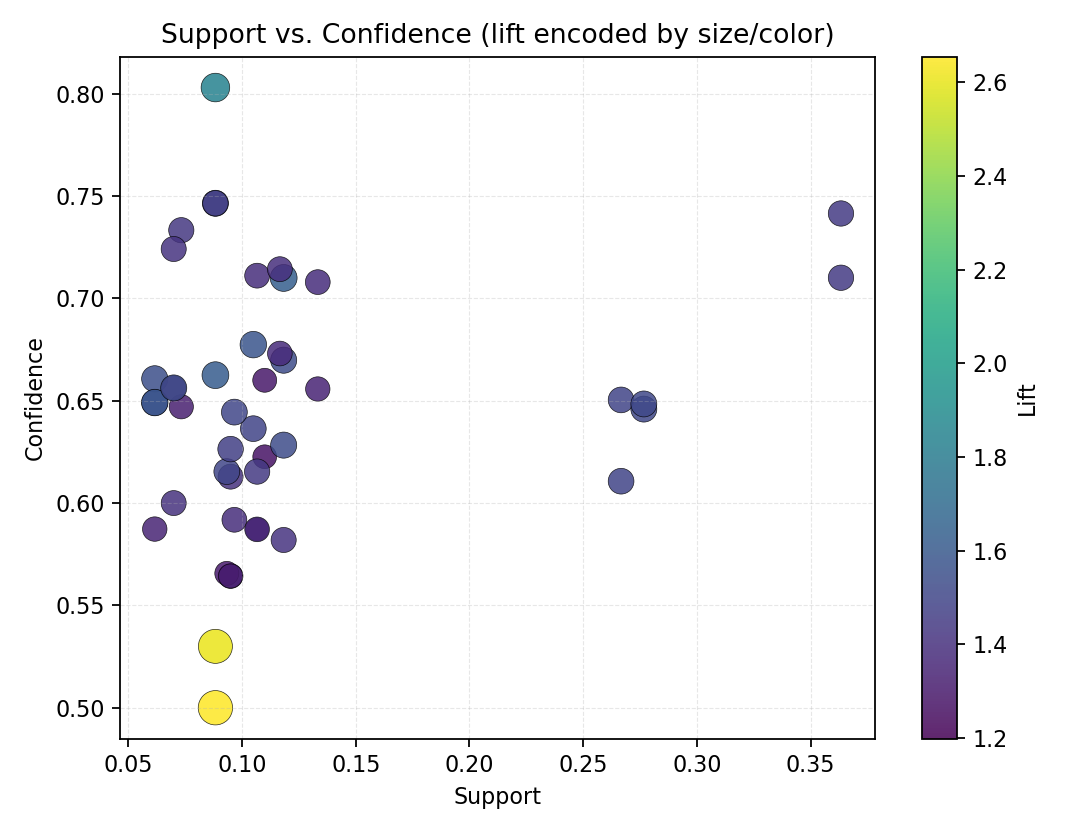
\includegraphics[width=0.82\linewidth]{fpgrowth_support_confidence.png}
  \caption{FP-Growth 规则的支持度-置信度散点图,点大小对应提升度}
  \label{fig:fpgrowth_support_confidence_cn}
\end{figure}

\begin{figure}[H]
  \centering
  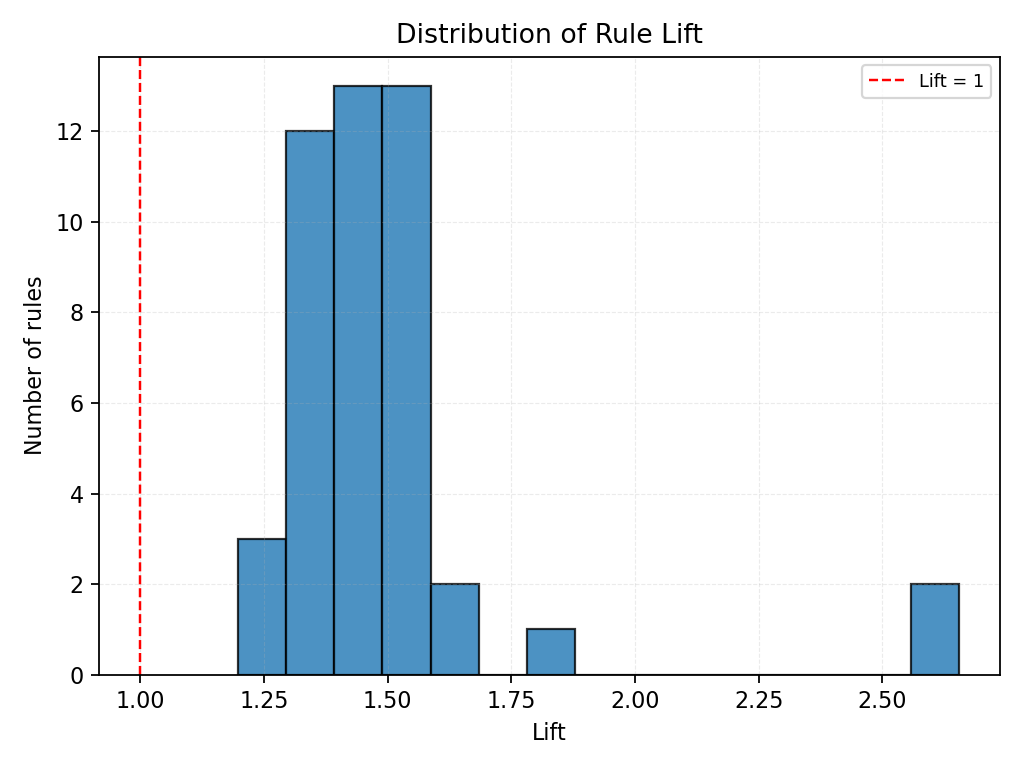
\includegraphics[width=0.78\linewidth]{fpgrowth_lift_distribution.png}
  \caption{提升度分布,突出高关联度规则}
  \label{fig:fpgrowth_lift_distribution_cn}
\end{figure}

\FloatBarrier
\section{总结}
FP-Growth 通过 FP-tree 与条件模式基避免暴力枚举频繁项集。只要合理设置支持度阈值、排序策略及评价指标,就能在大规模数据上高效挖掘可解释的关联规则。示例展示了如何利用可视化评估模式质量并调整参数。

\end{document}
